\documentclass{article}
\usepackage[utf8]{inputenc}
\title{Lecture 3 :HDFS}
\author{wbg231 }
\date{December 2022}
\newcommand{\R}{$\mathbb{R}$}
\newcommand{\B}{$\beta$}
\newcommand{\A}{$\alpha$}
\newcommand{\D}{\Delta}

\newcommand{\avector}[2]{(#1_2,\ldots,#1_{#2})}
\newcommand{\makedef}[2]{$\textbf{#1}$:#2 }
\usepackage{tikz,graphicx,hyperref,amsmath,amsfonts,amscd,amssymb,bm,cite,epsfig,epsf,url}

\begin{document}

\maketitle

\begin{itemize}
\item \href{https://brightspace.nyu.edu/d2l/le/lessons/261985/topics/8371478}{slides}
\section{last week and this week}
\item last time we took a look at map reduce which was a distributed computation system 
\item this week we will be discussing distributed storage, the Hadoop file System, HDFS and map reduce
\section{map reduce }
\subsection{simulating map reduce on a single machine}
\item 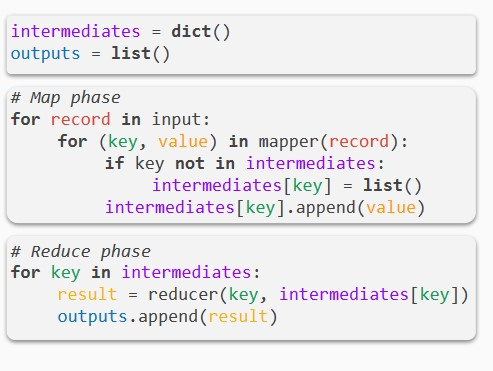
\includegraphics[width=10cm]{lecture notes/week_4/immages/l4_1.jpg}
\item so first an intermediate dictionary (ie key value pairs) and output list are created. 
\item then we enter the map phase
\begin{itemize}
    \item within the map phase we go over each record in our input file 
    \item then within each record we apply map(record)->(key,value)
    \item recall that the mapper takes a list an applies some operation to it element wise so it works like this $map(x_1...x_n)\rightarrow [(x_1,f(x_1)),...((x_n,f(x_n)) ]$
    \item then if the key value i not already in our dictionary we create a new empty list in our dictionary associated with that key and if it is we append to the list the value
\end{itemize}
\item then we hit the reduce phase
\begin{itemize}
    \item we go through each key in the intermediate 
    \item and run reducer(key,intermediates[key])
    \item recall that the reducer function takes a list and merges them all by some rule into an item 
    \item that item is then append into our outputs 
\end{itemize}
\item the question becomes how can we make this work across multiple machines at a single time?
\section{map reduce details}
\item important questions for working across multiple machines are:
\begin{enumerate}
    \item how is the data shared over the cluster
    \item how do we handle node failures?
    \item how can we optimize for amp reduce operations
\end{enumerate}
\item to answer this lets start simple
\begin{itemize}
    \item within map reduce the head node sends (mapper, reducer) code and a block of data to each worker
    \item the worker run the mapper on the data to get intermediate results, then the reducer on the intermediate results to get final results. then they send the output back to the head 
    \item problems
    \begin{itemize}
        \item this will work but it is inefficient 
        \item each job moves the entire dataset over the network. this can be thought of as a failure of locality
    \end{itemize}

\end{itemize}
\item so what if we localize all data 
\begin{itemize}
    \item suppose that all data was replicated on all worker nodes. 
    \itme the head would only need to send (mapper, reducer) and the id of a data block to each each worker 
    \item the worker would still need to run the mapper on the data to get intermediate results, then the reducer on the intermediate results to get final results. then they send the output back to the head 
\end{itemize}
\begin{itemize}
    \item this is also sub optimal 
    \item each worker stores a large amount of data they do not even use 
\end{itemize}
\item so in a ideal design we would like to keep the following things in mind  
\begin{itemize}
    \item communicate cost (ie how much data is being transfers)
    \item fault tolerance how comfortable are we with mistakes in our data or calculations 
    \item redundancy vs communication (ie should we store more data locally on worker nodes or have it sent)
    \item granularity of access
    \item locality
    \item common access patterns 
    \item programs are small, data is big. 
\end{itemize}
\section{hadoop}
\subsection{Hadoop distributed file systems}
\item HDFS is the storage component of Hadoop (it does more than just map reduce) 
\item provides distributed redundant storage
\item optimized for singe-write, multi read patters
\subsection{networked file systems (NFS) vs Hadoop's}
\item NFS stores data on one machine but provides access from multiple machines
\item HDFS spreads each file across multiple machines ~1 disk per machine with no internal redundancy
\item if a disk fails a machine needs to go offline either way. fault tolerance is at the level of machines, not disk. this lets us tolerate other machine level failures not just disk. 
\subsection{using HDFS}
\item HDFS is a file system but we use it differently
\item HDFS sits on top of the operating systems built in FS
\item it is better to think of it as an app that stores files for you kind of like good drive, can be accessed from bash with the hadoop fs command 
\item there are two types of nodes name and data nodes
\subsection{name nodes}
\item clients talk to the name nodes to locate data. it is analogous to the file system in a standard os
\item the name node knows the following mappings 
\begin{itemize}
    \item files $\rightarrow$ blocks
    \item blocks$\rightarrow $data
\end{itemize}
\item the name node keeps a running journal of transactions that is backed up and remotely distributed to avoid error
\subsection{data nodes}
\item store each block as two files in the local system 
\begin{itemize}
    \item the data block 
    \item and metadata which has :
    \begin{itemize}
        \item checksum used to detect storage errors. if the checksum is wrong the data is likely wrong  
        \item generation stamp which is used to detect updates to the data. 
    \end{itemize}
\end{itemize}

\subsection{example operation: writing to hdfs}
\item The read write looks like this \\ 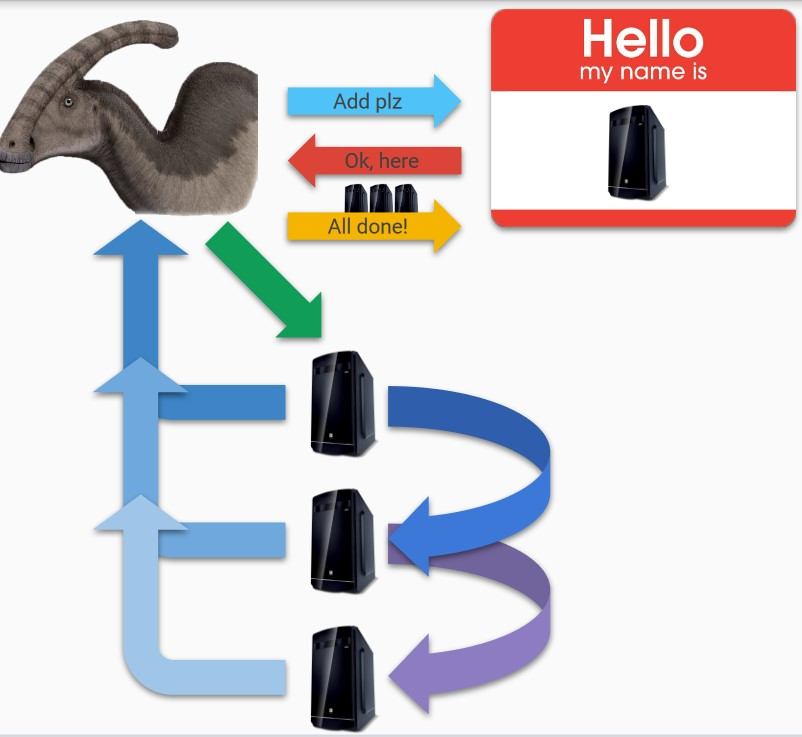
\includegraphics[width=10cm]{lecture notes/week_4/immages/l4_2.jpg}
\item so step 1 is the dinosaurs representing the user requests that a block should be added to memory.
\begin{itemize}
    
\item they communicate it to the name node. (blue arrow out from the dino) 
\item the name node then responds with a list of data nodes (red arrow out from teh name node)
\end{itemize}
\item step two
is the clinet or user sends the block ie infomraiton to the first data node. (green arrow)
\item step three
\begin{itemize}
    \item data node 1 stores the block ie data
    \item data node 1 ackowladges that it got the info (light blue arorw to user)
    \item data node 1 sends the data to data node 2
\end{itemize}
\item step 4
\begin{itemize}
    \item data node 2 stores the data
    \item data node 2 ackowledges that it got teh data light blue arrow to user
    \item data node 2 sends block to data node 3
\end{itemize}
\item step 5
\begin{itemize}
    \item   node 3 stores the data
    \item data node 3 ackowledges that it got teh data light blue arrow to user
\end{itemize}
\item step 6: the client knows it has gotten receipts from all data nodes and sends that the job is done to the name node (yellow arrow) 
\subsection{name and data node communication }
\item data nodes periodically signal the name node (called heart beats) every three seconds
\item the name node always knows which data nodes are alive ie active. it can infer a data node has failed if it does not get a heart beat 
\item the name node made respond with update messages. ie update instructions sent to data node
\section{failure tolerance}
\subsection{check points}
\item check points are snapshots of the current name nodes state including 
\begin{itemize}
    \item directory structure, block maps and journal (all kept in ram)
\end{itemize}
\item these are created periodically to ensure that the program can recover quickly from failure of the name node 
\item checkpoints cannot be updated only replaced. 
\subsection{HDFS is not POSIX Compliant}
\item POSIX is a standard for file systems that ensures they are easy to work with between operating systems \href{https://en.wikipedia.org/wiki/POSIX}{link}
\item updates are append only 
\begin{itemize}
    \item old data can not be changed only new data added.
    \item this makes it much easier to track changes, as well as replicate the changes
    \item 
\end{itemize}
\item not all file models are supported. the idea is to hold data so something like executable files or bash scripts don't really make sense
\section{HDFS not like desktop}
\item desktop computers need to support all kinds of uses. files need to be updated frequently 
\item large data analysis jobs have specific needs
\begin{itemize}
    \item there are a small number of large files
    \item to analyze data, files need to be read a lot 
    \item data rarely needs to be updated. ie append only writing is ok
\end{itemize}
\subsection{division of responsibility}
\item name nodes no not store data, they store metadata 
\item data nodes do not store meta data they store data 
\item name node failure can be catastrophic 
\item data not failure can be tolerated to a point depending on the level of replication 
\section{question}
\item why does HDFS parallels storage at the level of blocks instead of files ?
\item there are a few reasons 
\begin{itemize}
    \item a file can be larger than any single disk
    \item map reduce programs only work with small portions of large file
    \item uniform maximum block size makes allocation and replication very easy
\end{itemize}
\subsection{HDFS not POSIX-complied II}
\item portable operation system interface (POSIX) requires:
\begin{itemize}
    \item standard around os and file system compatibility 
    \item standard operations read write seek etc
\end{itemize}
\item HDFS updates are append only 
\begin{itemize}
    \item no changing old data 
    \item this makes replication logic much more simple 
\end{itemize}
\item not all file types are supported
\section{hadoop and map reduce}
\subsection{typical map reduce work flow }
\begin{enumerate}
    \item upload data from UNIX to HDFS
    \begin{itemize}
    \item hadoop fs - put $myile$.csv
\end{itemize}
\item run map reduce program 
\begin{itemize}
    \item each mapper sees a portion of myfile.csv
    \item each mapper produces intermediate outputs as hdfs files 
    \item shuffle stage collects intermediate outputs to give to reduces 
    \item reduces operate on intermediates produce final output as multiple blocks 
\end{itemize}
\item retrive output form HDFS
\begin{itemize}
    \item hadoop fs -getmerge myoutputfile.csv
\end{itemize}
\end{enumerate}
\subsection{hwo does HDFS help map reduce }
\item HDFS shares data blocks over data nodes (ie nodes hold data, and are told how to compute things) 
\item map reduce shares jobs over compute nodes (ie nodes hold computation and are given the data)
\item data is big computation is small, so sending computation instructions to nodes is cheaper than sending data institutions 
\subsection{job scheduling and input splits}
\item a typical map reduce job runs over only large file . each file contains an array of independent input
\item map reduce divides the input into splits. a split is a unit of work assigner to a mapper. each split might contain  multiple records
\item each split maps onto one or more block, usually try to assign work for a split such that machines can work on its block 
\item HDFS exposes block layout to the application layer to make this possible
\subsection{slido 2}
\item what will happen if a split is spread across multiple hdfs blocks? 
\item a split is one logical devision of the input data for a map process. ussualyl contianing multiple records like mulitple rows of a csv
\item machine nnuning mapper must have acess to the entire split, so data blocks may have to move to accomadate this 
\item by defualy split size=block size but there may be some framaentation, require more data movemnt adn thus slower compuation 
\subsection{where to run a split}
\item base case: exeexute the split on a node that stores the blocks we need 
\item okay case: excecute ona  difrent node in teh same rack that stores the block we need (within  rack comuncation is fast)
\item worst case: exceture on a node in a difrent rack. between rack communcation is the slowest. 
\subsection{replication factors}
\item if we copy a block to multiple nodes schedule splits becomes easier. we are more likely to find a free worker that has the block we want 
\item HDFS lets you set the replication factor for each file. replication is not free. cost is multiplicative with data size
\item typical setup is 3 times replication. if possible 2 nodes in one Rock and 1 in a separate wrack have each block. this protect both against node and rack failure
\section{cap and hdfs}
\subsection{the cap theorem of distributed storage}
\item Consistency (C) read always produces the most recent value 
\item Availability (a) requests cannot be ignored
\item partition-tolerance (p)- system maintains correctness during network failure
\item a database can only have 2 of these three properties which are all desirable for there own reasons 
\item \href{https://www.ibm.com/topics/cap-theorem}{further reading}
\subsection{why cant we have cap}
\item assume that we had a system with all three pretties
\begin{enumerate}
    \item m1 and m2 are initialized with x=0
    \item the network fails and x=1 only updates on m1 
    \item then we read x form m. 
\end{enumerate}
\item what happens next? 
\item if you want consistency then you must either give up availability or portion tolerance.
\item if you want availability then you must be ok with either loosing consistency or part ion tolerance 
\subsection{HDFS and CAP}
\item consistency 
\begin{itemize}
    \item centralized name node always has consistent view of the file system
    \item data can be added but not modified. 
\end{itemize}
\item availability
\begin{itemize}
    \item if the name node goes offline the system crashes 
\end{itemize}
\begin{itemize}
    \item depends on the network configuration and replication factor
\end{itemize}
\item so HDFS is consistent  
\item HDFS is part ion tolerant
\item availability how ever can fail
\item \href{https://stackoverflow.com/questions/58796173/how-does-the-cap-theorem-apply-on-hdfs}{more info}
\subsection{updates to HDFS since the 2010 paper}
\item now there can be multiple name nodes within the same HDFS which each mange part of the file system 
\item there are now standby nodes that can step in if a node fails emaning no single point of failure 
\itme 

\end{itemize}
\end{document}
